%%%%%%%%%%%%%%%%%%%%%%%%%%%%%%%%%%%%%%%%%%%%%%%%%%%%%%%%%%%%%%%%%%%%%%%%%%%%%%%%%%%%%%%%%%%%%%%%%%%
\newpage
\section{Introducción}
%%%%%%%%%%%%%%%%%%%%%%%%%%%%%%%%%%%%%%%%%%%%%%%%%%%%%%%%%%%%%%%%%%%%%%%%%%%%%%%%%%%%%%%%%%%%%%%%%%%

Se define herencia como el proceso mediante el cual una clase adquiere las propiedades (atributos) y comportamientos (métodos) de otra clase. 

En programación orientada a objetos comprender los conceptos de herencia, polimorfismo, funciones virtuales y sobrecarga es de vital importancia para lograr aplicar el concepto de clases a la resolución de diferentes tipos de problemas en las que usar estos conceptos nos ayuda a modelar la solución de una manera más eficiente y adecuada. 

%%%%%%%%%%%%%%%%%%%%%%%%%%%%%%%%%%%%%%%%%%%%%%%%%%%%%%%%%%%%%%%%%%%%%%%%%%%%%%%%%%%%%%%%%%%%%%%%%%%
\subsection{Objetivos}
\begin{enumerate}
\item Repasar y utilizar los conceptos de herencia, polimorfismo y sobrecarga. 
\item Practicar la sobrecarga de operadores para simplificar algunas operaciones.
\item Realizar un diagrama UML que permita visualizar la relación entre clases. 
\end{enumerate}
%%%%%%%%%%%%%%%%%%%%%%%%%%%%%%%%%%%%%%%%%%%%%%%%%%%%%%%%%%%%%%%%%%%%%%%%%%%%%%%%%%%%%%%%%%%%%%%%%%%
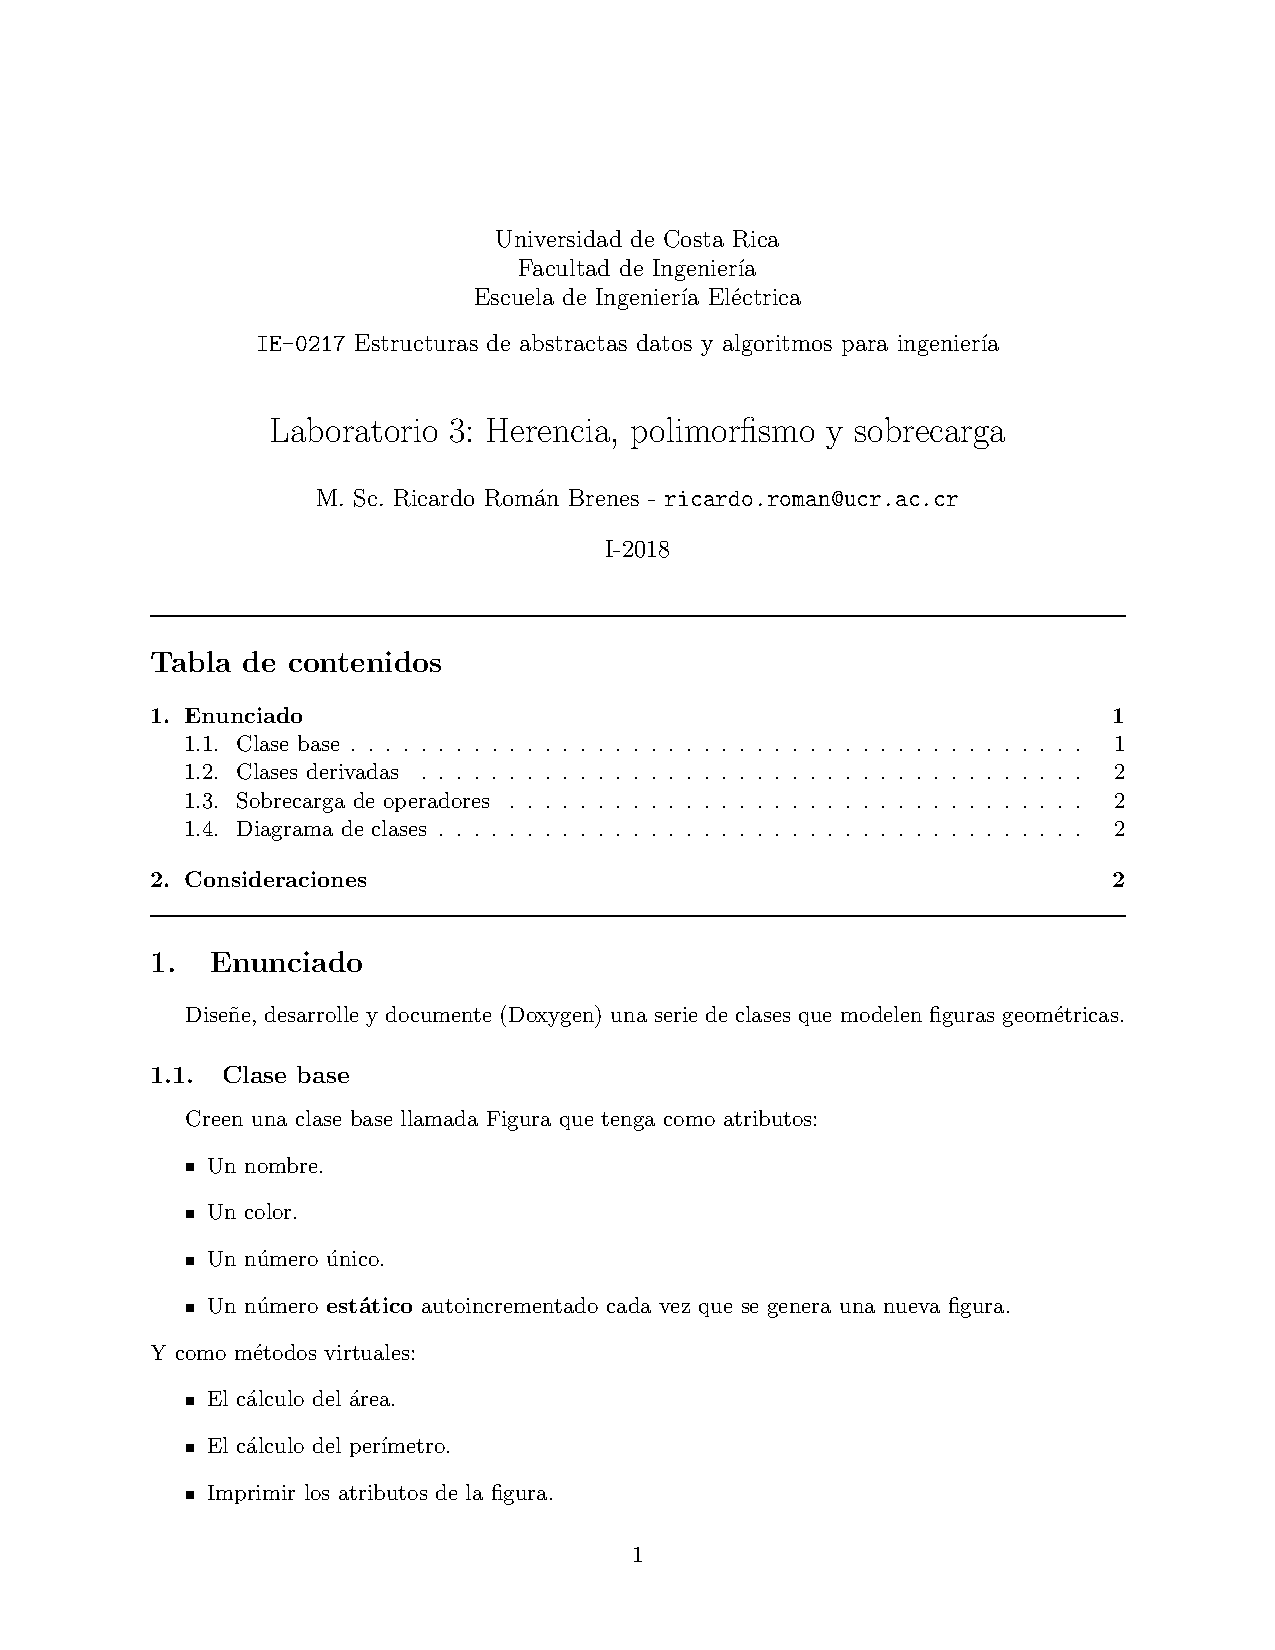
\includepdf[pages=1,pagecommand=\section{Enunciado}]{enunciados/enun3}
\includepdf[pages=2,pagecommand={}]{enunciados/enun3}
%%%%%%%%%%%%%%%%%%%%%%%%%%%%%%%%%%%%%%%%%%%%%%%%%%%%%%%%%%%%%%%%%%%%%%%%%%%%%%%%%%%%%%%%%%%%%%%%%%%

%%%%%%%%%%%%%%%%%%%%%%%%%%%%%%%%%%%%%%%%%%%%%%%%%%%%%%%%%%%%%%%%%%%%%%%%%%%%%%%%%%%%%%%%%%%%%%%%%%%
\section{Solución}
%\begin{minted}[linenos,autogobble,bgcolor=bg,breaklines,fontsize=\footnotesize ]{c++}

%\end{minted}
%%%%%%%%%%%%%%%%%%%%%%%%%%%%%%%%%%%%%%%%%%%%%%%%%%%%%%%%%%%%%%%%%%%%%%%%%%%%%%%%%%%%%%%%%%%%%%%%%%%
\subsection{Clase base: \texttt{Figure()}}
La clase \texttt{Figure()} es la clase base del programa, de donde las demás clases heredan. En el \textit{header} \texttt{Figure.h} se definen los métodos y atributos de la clase. En la sección pública se colocan las definiciones de los métodos constructor, destructor, así como los métodos virtuales para calcular el área, el perímetro, y la función encargada de imprimir los datos de la clase. Se declaran los atributos como protegidos, en estos se incluye el nombre, el color, un número único para el objeto, y un número estático que se incrementa cada vez que se genera una figura, para esto se implementa un método más.

\begin{minted}[linenos,autogobble,bgcolor=bg,breaklines,fontsize=\footnotesize ]{c++}
#include <string>
#include <iostream>
using namespace std;
#ifndef FIGURE_H
#define FIGURE_H

///@class Figure
class Figure {
  public:
    Figure();
    ~Figure();
    virtual double area() = 0 ; 
    virtual double perimetro() = 0; 
    virtual void imprimir() = 0;
  protected:
    int getNumAutoInc();
    string nombre;
    string color;
    int numUnico;
    static int numAutoInc; 
  private:
};
#endif
\end{minted}

\subsection{Clase derivada: \texttt{Rectangle()}}

La clase \texttt{Rectangle()} hereda de la clase base; como se observa a la hora de declararlo mediante la línea \texttt{class Rectangle : public Figure}. En el archivo \texttt{Rectangle.h} se observan los métodos que contiene esta clase. Para los cálculos respectivos a un rectángulo, se declaran dos variables protegidas de tipo \texttt{double} para almacenar el largo y el ancho de la figura.
\begin{minted}[linenos,autogobble,bgcolor=bg,breaklines,fontsize=\footnotesize ]{c++}
#include <string>
#include <iostream>
#include "../include/Figure.h"
using namespace std;
#ifndef RECTANGLE_H
#define RECTANGLE_H

///@class Rectangle
class Rectangle : public Figure {
  public:
    Rectangle();
    Rectangle(string nombre, string color, int numUnico, double largo, double ancho);
    Rectangle(const Rectangle& r);
    ~Rectangle();
    double area();
    double perimetro();
    void imprimir();
    void operator~();
    void operator!();
    void operator=(const Rectangle& r);
  protected:
    double largo;
    double ancho;
  private:
};
#endif
\end{minted}

\subsubsection{Métodos de \texttt{Rectangle()}}
\begin{itemize}
\item \textbf{Constructor vacío:}

	Cuando se crea un objeto de tipo \texttt{Rectangle} sin pasarle ningún argumento, se utiliza este constructor. Aquí se le solicita al usuario que ingrese los datos necesarios para crear el objeto con sus atributos bien definidos. Se solicita el nombre, el color, el número único y las medidas de los lado, todo lo anterior se guarda en las variables de los atributos respectivos utilizando el operador \texttt{this->}.
    \begin{minted}[linenos,autogobble,bgcolor=bg,breaklines,fontsize=\footnotesize ]{c++}
Rectangle::Rectangle(){
  cout << endl <<"Ingrese el nombre del rectangulo:  ";
  cin >> this->nombre;
  cout << endl << "Ingrese el color del rectangulo:  ";
  cin >> this->color;
  cout << endl << "Ingrese un numero unico para identificar el rectangulo:  ";
  cin >> this->numUnico;
  cout << endl << "Ingrese la medidad del lado largo del rectangulo:  ";
  cin >> this->largo;
  cout << endl << "Ingrese la medidad del ancho del rectangulo:  ";
  cin >> this->ancho;
}   
    \end{minted}
    
\item \textbf{Constructor con parámetros:}

	El constructor con parámetros se utiliza cuando se crea un objeto y se le pasan los atributos como argumentos al método.
	\begin{minted}[linenos,autogobble,bgcolor=bg,breaklines,fontsize=\footnotesize ]{c++}
Rectangle::Rectangle(string nombre, string color, int numUnico, double largo, double ancho) {
  this->nombre = nombre;
  this->color = color;
  this->numUnico = numUnico;
  this->largo = largo;
  this->ancho = ancho;
}
   \end{minted}

\item \textbf{Constructor por copia:}

Para crear un objeto inicializándolo con otro ya existente. Se pasa una referencia al objeto existente, y se copian sus atributos en el nuevo objeto.

\begin{minted}[linenos,autogobble,bgcolor=bg,breaklines,fontsize=\footnotesize ]{c++}
Rectangle::Rectangle(const Rectangle &copyRectangle){
  this->nombre    = copyRectangle.nombre;
  this->color     = copyRectangle.color;
  this->numUnico  = copyRectangle.numUnico;
  this->largo     = copyRectangle.largo;
  this->ancho     = copyRectangle.ancho;
}
\end{minted}

\item \textbf{Área y perímetro:}

	Los dos métodos para calcular el área y el perímetro simplemente en el \texttt{return} realizan la operación necesaria para obtener el resultado. Para obtener las medidas de los lados se utilizan los atributos utilizando el puntero \texttt{this->}. Por el tipo de cálculo a realizar, las funciones devuelven el resultado tipo \texttt{double}.
    
	\begin{minted}[linenos,autogobble,bgcolor=bg,breaklines,fontsize=\footnotesize ]{c++}
double Rectangle::area(){
  return (this->largo*this->ancho);
}
\end{minted}

	\begin{minted}[linenos,autogobble,bgcolor=bg,breaklines,fontsize=\footnotesize ]{c++}
double Rectangle::perimetro(){
  return ((2*(this->largo))+(2*(this->ancho)));
}
\end{minted}

\item \textbf{Método imprimir:}

	Imprime todos los datos del objeto.
    	\begin{minted}[linenos,autogobble,bgcolor=bg,breaklines,fontsize=\footnotesize ]{c++}
void Rectangle::imprimir() {
  cout << "Nombre: " << this->nombre << endl;
  cout << "Color: " << this->color << endl;
  cout << "Número Único: " << this->numUnico << endl;
  cout << "Largo: " << this->largo << endl;
  cout << "Ancho: " << this->ancho << endl;
  cout << "Número Autoincrementado: " << this->numAutoInc << endl;
}
\end{minted}

\item \textbf{Sobrecarga de operadores}\\
Se implementa la sobrecarga de los operadores \texttt{!, \~} y \texttt{=}. El operador \texttt{!} se utiliza para calcular el área y el perímetro; \texttt{\~} se utiliza para imprimir los datos del objeto, y el operador \texttt{=} se utiliza para igualar o copiar un objeto en otro.

\begin{minted}[linenos,autogobble,bgcolor=bg,breaklines,fontsize=\footnotesize ]{c++}
void Rectangle::operator~(){
  imprimir();
}
void Rectangle::operator!(){
  cout << "Area: " << area() << endl;
  cout << "Perimetro: " << perimetro() << endl;
}
void Rectangle::operator=(const Rectangle& r)
{
  this->nombre    = r.nombre;
  this->color     = r.color;
  this->numUnico  = r.numUnico;
  this->largo     = r.largo;
  this->ancho     = r.ancho;
}
\end{minted}


\end{itemize}



\subsection{Clase derivada: \texttt{Triangle()}}

\begin{minted}[linenos,autogobble,bgcolor=bg,breaklines,fontsize=\footnotesize ]{c++}
#include <string>
#include <iostream>
#include "../include/Figure.h"
#ifndef TRIANGLE_H
#define TRIANGLE_H

class Triangle : public Figure
{
  public:
    Triangle();
    Triangle(string n, string c, int num, double l1, double l2, double l3);
    Triangle(const Triangle& r);
    ~Triangle();
    double area();
    double perimetro();
    void imprimir();
    void operator~();
    void operator!();
    void operator=(const Triangle& t);
  private:
	  double lado1;
	  double lado2;
	  double lado3;
	  string tipo;	//tipo de triangulo
	  void initIDs();	//para pedir valores de atributos al usuario
  	void initLados(); //para pedir valores de los lados al usuario
  	bool desigualdad(double a, double b, double c); //teorema de la desigualdad para ver si con lados ingresados se puede formar un triangulo
  	bool verifLados(double l1, double l2, double l3);
  	void verifTipo(double l1, double l2, double l3);
  };

#endif

\end{minted}

\subsubsection{Métodos de \texttt{Triangle()}}

\begin{itemize}
\item \textbf{Constructor vacío:}\\
Si se crea una instancia de \texttt{Triangle} utilizando el constructor vacío, se llamará a los métodos que se encargan de inicializar los atributos correspondientes. De esta manera, no se permite que existan objetos sin alguno de los atributos asignado.
\begin{minted}[linenos,autogobble,bgcolor=bg,breaklines,fontsize=\footnotesize ]{c++}
Triangle::Triangle(){
	initIDs();
	initLados();
	verifTipo(this->lado1,this->lado2,this->lado3);
}
\end{minted}

\item \textbf{Constructor con parámetros:}\\
Se puede crear un objeto \texttt{Triangle} pasándole los atributos en el constructor, en un orden específico. En este caso, se debe llamar a un método que verifica si los lados con los que se desea construir este objeto son válidos (más adelante se explica de qué se trata esto).
\begin{minted}[linenos,autogobble,bgcolor=bg,breaklines,fontsize=\footnotesize ]{c++}
Triangle::Triangle(string n, string c, int num, double l1, double l2, double l3){
	if (verifLados(l1,l2,l3) == false){
		initLados();
	}
	else {
		this->lado1 = l1;
		this->lado2 = l2;
		this->lado3 = l3;
	}
	this->nombre = n;
	this->color = c;
	this->numUnico = num;
	verifTipo(this->lado1,this->lado2,this->lado3);
}
\end{minted}

\item \textbf{Constructor por copia:}\\
Para crear un objeto inicializándolo con otro ya existente. Se pasa una referencia al objeto existente. 

\begin{minted}[linenos,autogobble,bgcolor=bg,breaklines,fontsize=\footnotesize ]{c++}
Triangle::Triangle(const Triangle &copy){
  this->nombre    = copy.nombre;
  this->color     = copy.color;
  this->numUnico  = copy.numUnico;
  this->lado1     = copy.lado1;
  this->lado2     = copy.lado2;
  this->lado3     = copy.lado3;
  this->tipo      = copy.tipo;
}
\end{minted}


\item \textbf{Inicializador de identificadores (\texttt{initIDs()})}\\
Así se denominó al método que solicita al usuario los valores de los atributos \texttt{nombre}, \texttt{color} y \texttt{numUnico}, para asignárselos al objeto creado. No se hace verificación de tipos. 

\begin{minted}[linenos,autogobble,bgcolor=bg,breaklines,fontsize=\footnotesize ]{c++}
void Triangle::initIDs(){
	string n, c;
	int num;
	cout << endl << "Ingrese el nombre del triangulo:  ";
	cin >> n;
	cout << endl << "Ingrese el color del triangulo:  ";
	cin >> c;
	cout << endl << "Ingrese un numero unico para identificar el triangulo: ";
	cin >> num;
	this->nombre = n;
	this->color = c;
	this->numUnico = num;
}
\end{minted}

\item \textbf{Método \texttt{initLados()}}\\
Solicita al usuario los valores de los lados, de tipo \texttt{double}. Antes de asignarle estos valores al objeto creado, utiliza el método \texttt{verifLados()} para determinar si son valores válidos. El ciclo \texttt{do ... while} permite ejecutar la solicitud al usuario, y luego verificar si se cumple la condición; de no ser así, la solicitud se vuelve a realizar.

\begin{minted}[linenos,autogobble,bgcolor=bg,breaklines,fontsize=\footnotesize ]{c++}
void Triangle::initLados(){
	double l1, l2, l3;
	do {
		cout << endl <<"Ingrese el primer lado: ";
		cin >> l1;
		cout << endl << "Ingrese el segundo lado:  ";
		cin >> l2;
		cout << endl << "Ingrese el tercer lado:  ";
		cin >> l3;
	} while (verifLados(l1,l2,l3)==false);
	this->lado1 = l1;
	this->lado2 = l2;
	this->lado3 = l3;
}
\end{minted}

\item \textbf{Método \texttt{verifLados()}}\\
Este método verifica si los valores que se quiere asignar a los lados del triángulo creado, son valores válidos; esto es, si cumplen el teorema de la desigualdad triangular. Este teorema establece que los lados l1, l2 y l3 forman un triángulo si la suma de cualesquiera dos de ellos es mayor al lado restante. Este teorema se implementa aquí con otro método llamado \texttt{desigualdad()}, que retorna un valor booleano. Se indica en un mensaje si los lados ingresados son válidos.

\begin{minted}[linenos,autogobble,bgcolor=bg,breaklines,fontsize=\footnotesize ]{c++}
bool Triangle::verifLados(double l1, double l2, double l3){
	if (desigualdad(l1,l2,l3) == true){
		cout << endl << "Lados válidos" << endl << endl;
		return true;
	}
	else{
		cout << endl<< "Los lados ingresados (" << l1 << "," << l2 << "," << l3 << ") no pueden formar un triángulo. Ingrese lados válidos." << endl;
		return false;
	}
}

bool Triangle::desigualdad(double a, double b, double c){
	if ((a<b+c) && (b<a+c) && (c<a+b)){
		return true;
	}
	else {
		return false;
	}
}
\end{minted}

\item \textbf{Método \texttt{verifTipo()}}\\
Evalúa los lados del triángulo para determinar si este es ``equilátero'', ``isósceles'' o ``escaleno'', y asigna el valor resultante al atributo \texttt{tipo}.

\begin{minted}[linenos,autogobble,bgcolor=bg,breaklines,fontsize=\footnotesize ]{c++}
void Triangle::verifTipo(double l1, double l2, double l3){
	if (l1 == l2 && l2 == l3){
		this->tipo="equilatero";
	}
	else if ((l1==l2)||(l1==l3)||(l2==l3)){
		this->tipo="isosceles";
	}
	else {
		this->tipo="escaleno";
	}
}
\end{minted}

\item \textbf{Métodos \texttt{perimetro()} y \texttt{area()}}\\
El método \texttt{perimetro()} devuelve la suma de los lados, mientras que \texttt{area()} calcula el área a partir de los lados utilizando la fórmula de Herón:

\begin{equation}
A = \sqrt[]{s(s-a)(s-b)(s-c)}
\end{equation}

Donde $s$ es el valor del semiperímetro, es decir, la mitad del valor retornado por \texttt{perimetro()}. Para este cálculo se utilizó la función \texttt{sqrt()} de la biblioteca \texttt{math.c}. 

\begin{minted}[linenos,autogobble,bgcolor=bg,breaklines,fontsize=\footnotesize ]{c++}
double Triangle::perimetro(){
	return (this->lado1+this->lado2+this->lado3);
}

double Triangle::area(){
	double a = this->lado1, b = this->lado2, c = this->lado3;
	double semip = perimetro()/2;
	double heron = (semip*(semip-a)*(semip-b)*(semip-c));
	return sqrt(heron);
}
\end{minted}

\item \textbf{Método \texttt{imprimir()}}\\
Imprime en pantalla todos los atributos del objeto.

\begin{minted}[linenos,autogobble,bgcolor=bg,breaklines,fontsize=\footnotesize ]{c++}
void Triangle::imprimir() {
	cout << "Nombre: " << this->nombre << endl;
	cout << "Color: " << this->color << endl;
	cout << "Número Único: " << this->numUnico << endl;
	cout << "Tipo: " << this->tipo << endl;
	cout << "Lado 1: " << this->lado1 << endl;
	cout << "Lado 2: " << this->lado2 << endl;
	cout << "Lado 3: " << this->lado3 << endl;
	cout << "Número Autoincrementado: " << this->numAutoInc << endl;
}
\end{minted}

\item \textbf{Sobrecarga de operadores}\\
Se implementa la sobrecarga de los operadores \texttt{!, \~} y \texttt{=}.

\begin{minted}[linenos,autogobble,bgcolor=bg,breaklines,fontsize=\footnotesize ]{c++}
void Triangle::operator~(){
  imprimir();
}

void Triangle::operator!(){
  cout << "Area: " << area() << endl;
  cout << "Perimetro: " << perimetro() << endl;
}

void Triangle::operator=(const Triangle& t){
  this->nombre		= t.nombre;
  this->color		= t.color;
  this->numUnico	= t.numUnico;
  this->lado1		= t.lado1;
  this->lado2		= t.lado2;
  this->lado3		= t.lado3;
  this->tipo		= t.tipo;
}
\end{minted}

\end{itemize}

\subsection{Clase derivada: \texttt{Circle()}}
Como se observa a la hora de declarar la clase mediante la línea \texttt{class Circle : public Figure}, la clase \texttt{Circle()} hereda de la clase base. En el archivo \texttt{Circle.h} se observan los métodos que contiene esta clase. Para los cálculos respectivos del círculo, se declara una variable privada de tipo \texttt{double} para almacenar el radio de la figura.

\subsubsection{Métodos de \texttt{Circle()}}
\begin{minted}[linenos,autogobble,bgcolor=bg,breaklines,fontsize=\footnotesize ]{c++}
#include <string>
#include <iostream>
#include "../include/Figure.h"
using namespace std;
#ifndef CIRCLE_H
#define CIRCLE_H

class Circle : public Figure
{
  public:
    Circle();
    Circle(string nombre, string color, int numUnico, double radio);
    // Circle(const Circle& r);
    ~Circle();
    double area();
    double perimetro();
    void imprimir();
    void operator~();
    void operator!();
    void operator=(const Circle& r);
    //void operator=(Circle r);
  protected:
  private:
    double radio;
};
#endif
\end{minted}

\begin{itemize}
\item \textbf{Métodos constructores:}

	Para crear un nuevo objeto de tipo \texttt{Circle} se implementaron dos constructores, uno de ellos vacío que conforme se ejecuta se le piden al usuario los valores de los atributos del objeto. El otro constructor recibe como argumentos los parámetros mencionados. También se implementa el constructor por copia.
    
\begin{minted}[linenos,autogobble,bgcolor=bg,breaklines,fontsize=\footnotesize ]{c++}
Circle::Circle()
{
  cout << endl <<"Ingrese el nombre del círculo: ";
  cin >> this->nombre;
  cout << endl << "Ingrese el color del círculo: ";
  cin >> this->color;
  cout << endl << "Ingrese un número único para identificar el círculo: ";
  cin >> this->numUnico;
  cout << endl << "Ingrese la medida del radio del círculo: ";
  cin >> this->radio;
}
Circle::Circle(string nombre, string color, int numUnico, double radio)
{
  this->nombre    = nombre;
  this->color     = color;
  this->numUnico  = numUnico;
  this->radio     = radio;
}
\end{minted}

\item \textbf{Área y perímetro:}

	Los dos métodos para calcular el área y el perímetro simplemente en el \texttt{return} realizan la operación necesaria para obtener el resultado. Para obtener las medidas de los lados se utilizan los atributos utilizando el puntero \texttt{this->}. Por el tipo de cálculo a realizar, las funciones devuelven el resultado tipo \texttt{double}. Es importante destacar que para el cálculo del área se debe multiplicar por $\pi$, por lo que se define al inicio del archivo utilizando \texttt{\#define}.
    
	\begin{minted}[linenos,autogobble,bgcolor=bg,breaklines,fontsize=\footnotesize ]{c++}
    #define PI 3.14159265358979323846
\end{minted}
    
	\begin{minted}[linenos,autogobble,bgcolor=bg,breaklines,fontsize=\footnotesize ]{c++}
double Circle::area()
{
  return (PI*this->radio*this->radio);
}
\end{minted}

	\begin{minted}[linenos,autogobble,bgcolor=bg,breaklines,fontsize=\footnotesize ]{c++}
double Circle::perimetro()
{
  return (2.0*this->radio*PI);
}
\end{minted}

\item \textbf{Método imprimir y sobrecarga de los operadores \texttt{=} , \texttt{!} , \texttt{\~} :}

Al igual que en las clases anteriores se implementa un método para imprimir los datos del objetos. Además los operadores se definen para imprimir los datos del objeto, para calcular el área y el perímetro, y para igual o crear una copia de un objeto.

\begin{minted}[linenos,autogobble,bgcolor=bg,breaklines,fontsize=\footnotesize ]{c++}
void Circle::imprimir()
{
  cout << "Nombre: " << this->nombre << endl;
  cout << "Color: " << this->color << endl;
  cout << "Número Único: " << this->numUnico << endl;
  cout << "Radio: " << this->radio << endl;
  cout << "Número Autoincrementado: " << this->numAutoInc << endl;
}
\end{minted}
\begin{minted}[linenos,autogobble,bgcolor=bg,breaklines,fontsize=\footnotesize ]{c++}
void Circle::operator~()
{
  imprimir();
}
void Circle::operator!()
{
  cout << "Area: " << area() << endl;
  cout << "Perimetro: " << perimetro() << endl;
}
void Circle::operator=(const Circle& r)
{
  this->nombre    = r.nombre;
  this->color     = r.color;
  this->numUnico  = r.numUnico;
  this->radio     = r.radio;
}
\end{minted}


\end{itemize}

\subsection{Diagrama de clases.}
En la Figura \ref{fig:dia} se puede observar el diagrama de las clases implementadas. Las clases derivadas \texttt{Rectangle}, \texttt{Triangle} y \texttt{Circle} heredan de la clase base \texttt{Figure}, como se observa en la Figura \ref{fig:dia} mediante una flecha. Además se pueden observar los atributos y métodos que conforman cada una de ellas.
\begin{figure}[H]
  \centering
    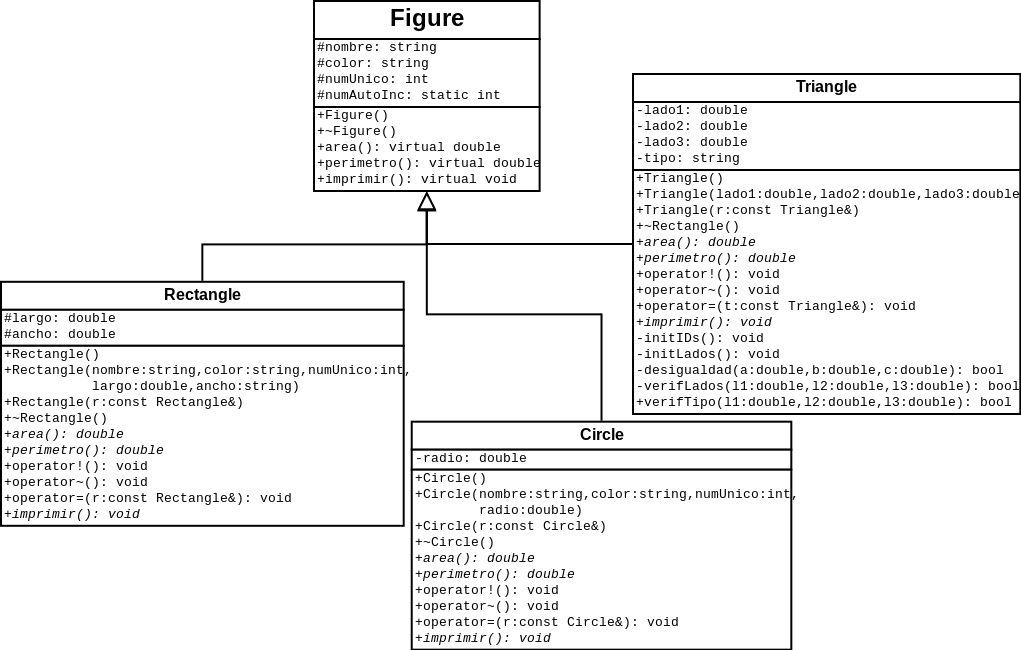
\includegraphics[width=\textwidth]{imgs/Labo3/Diagram1.png}
  \caption{Diagrama de clases}
  \label{fig:dia}
\end{figure}

%%%%%%%%%%%%%%%%%%%%%%%%%%%%%%%%%%%%%%%%%%%%%%%%%%%%%%%%%%%%%%%%%%%%%%%%%%%%%%%%%%%%%%%%%%%%%%%%%%%
\newpage
\section{Resultados}
%%%%%%%%%%%%%%%%%%%%%%%%%%%%%%%%%%%%%%%%%%%%%%%%%%%%%%%%%%%%%%%%%%%%%%%%%%%%%%%%%%%%%%%%%%%%%%%%%%%
Para observar los resultados de la implementación de las clases descritas, se creó un programa \texttt{main} en el que se crean algunos objetos. 

Para comprobar la funcionalidad de la clase \texttt{Circle}, se crea un objeto con el constructor vacío, lo cual causa que el programa solicite al usuario que ingrese los valores de los atributos:

\begin{minted}[linenos,autogobble,bgcolor=bg,breaklines,fontsize=\footnotesize ]{c++}
Circle circulo1 = Circle();
\end{minted}

Luego de esto se imprime los datos de información de la figura, área y perímetro, haciendo uso de la sobrecarga de los operadores $!$ y $\sim$. Posteriormente, se crea otra clase, pero esta vez pasándole los parámetros de los atributos a través del constructor:

\begin{minted}[linenos,autogobble,bgcolor=bg,breaklines,fontsize=\footnotesize ]{c++}
Circle circulo2("Circulo #2","Rojo",3,3.4);
\end{minted}

Por último, se comprueba el resultados de sobrecargar el operador = al igualar el primer circulo creado con el segundo. Los resultados de estas pruebas se pueden ver en la Figura \ref{fig:CIRC}.

\begin{figure}[H]
\centering
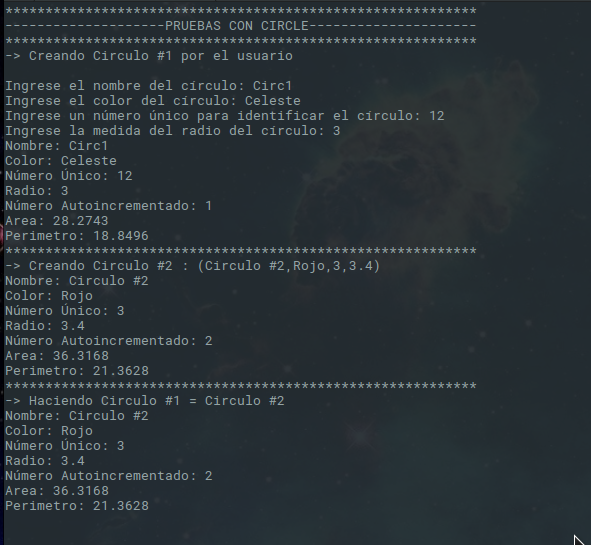
\includegraphics[width=.7\textwidth]{imgs/Labo3/CIRC}
\caption{Resultado de la implementación de la clase \texttt{Circle}}
\label{fig:CIRC}
\end{figure}

Una prueba similar se realizó para comprobar las funcionalidad de la clase \texttt{Rectangle} y los resultados se pueden ver en la Figura \ref{fig:RECT}.

\begin{figure}[H]
\centering
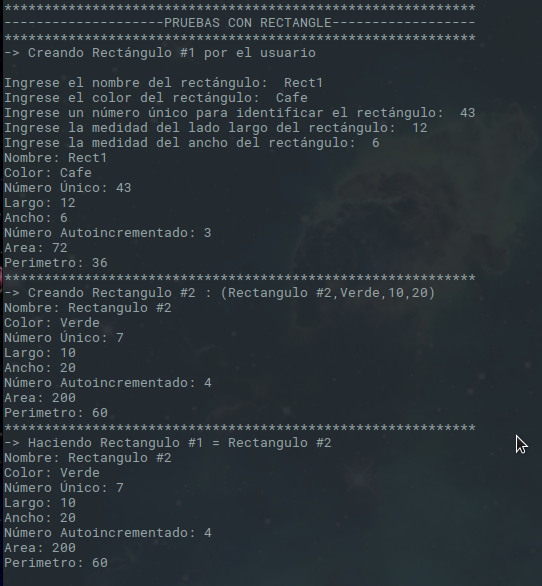
\includegraphics[width=.7\textwidth]{imgs/Labo3/RECT}
\caption{Resultado de la implementación de la clase \texttt{Rectangle}}
\label{fig:RECT}
\end{figure}

En la clase \texttt{Triangle}, también se hace una verificación para comprobar que los datos ingresados son válidos. En la Figura \ref{fig:TRI1}, se logra observar que si se ingresa lados que no cumplen para ser un triángulo, se solicita al usuario volver a ingresar datos.

\begin{figure}[H]
\centering
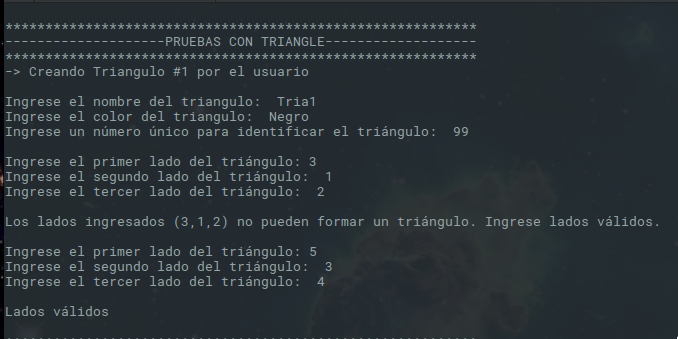
\includegraphics[width=.7\textwidth]{imgs/Labo3/TRI1}
\caption{Resultado de la implementación de la clase \texttt{Triangle}}
\label{fig:TRI1}
\end{figure}

Por último, se realizó la misma que para el círculo y rectángulo y los resultados se pueden ver en la Figura \ref{fig:TRI2}.

\begin{figure}[H]
\centering
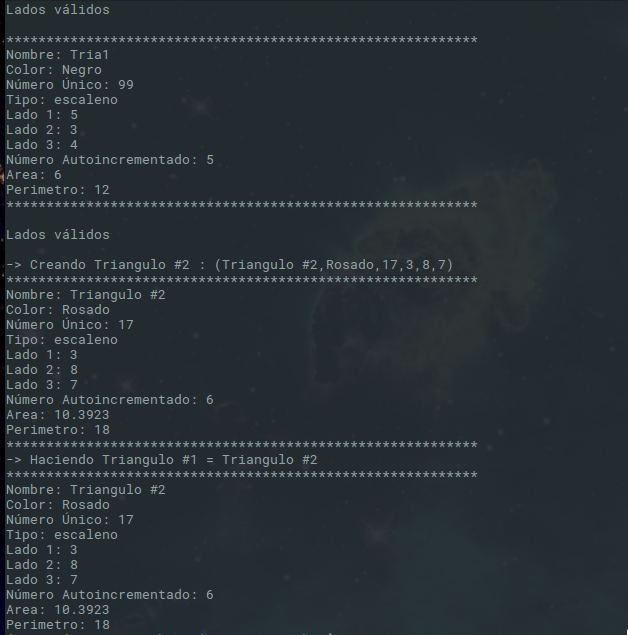
\includegraphics[width=.7\textwidth]{imgs/Labo3/TRI2}
\caption{Resultado de la implementación de la clase \texttt{Triangle}}
\label{fig:TRI2}
\end{figure}

Para correr toda la prueba es necesario ejecutar en la terminal el siguiente comando:

\begin{minted}[linenos,autogobble,bgcolor=bg,breaklines,fontsize=\footnotesize ]{bash}
make test
\end{minted}

%%%%%%%%%%%%%%%%%%%%%%%%%%%%%%%%%%%%%%%%%%%%%%%%%%%%%%%%%%%%%%%%%%%%%%%%%%%%%%%%%%%%%%%%%%%%%%%%%%%
\newpage
\section{Conclusiones}
 Como conclusiones se tiene que:
 
\begin{itemize}
\item A partir de una clase base se logra crear clases derivadas que contienen métodos y atributos heredados de la clase base, con esto se logra comprender el concepto de herencia en programación orientada a objetos.
\item Se implementó cuatro clases, con las cuales se logra crear círculos, rectángulos y triángulos y calcular su respectiva área y perímetro. 
\item Se logra sobrecargar operadores para darles diferentes usos y simplificar así la notación de las operaciones con objetos.
\item Se crea un diagrama UML con ejemplifica de mejor manera la jerarquía de las cuatro clases creadas en este proyecto.
\end{itemize}
%%%%%%%%%%%%%%%%%%%%%%%%%%%%%%%%%%%%%%%%%%%%%%%%%%%%%%%%%%%%%%%%%%%%%%%%%%%%%%%%%%%%%%%%%%%%%%%%%%%
